% Options for packages loaded elsewhere
\PassOptionsToPackage{unicode}{hyperref}
\PassOptionsToPackage{hyphens}{url}
\PassOptionsToPackage{dvipsnames,svgnames,x11names}{xcolor}
%
\documentclass[
  letterpaper,
  DIV=11,
  numbers=noendperiod]{scrreprt}

\usepackage{amsmath,amssymb}
\usepackage{iftex}
\ifPDFTeX
  \usepackage[T1]{fontenc}
  \usepackage[utf8]{inputenc}
  \usepackage{textcomp} % provide euro and other symbols
\else % if luatex or xetex
  \usepackage{unicode-math}
  \defaultfontfeatures{Scale=MatchLowercase}
  \defaultfontfeatures[\rmfamily]{Ligatures=TeX,Scale=1}
\fi
\usepackage{lmodern}
\ifPDFTeX\else  
    % xetex/luatex font selection
\fi
% Use upquote if available, for straight quotes in verbatim environments
\IfFileExists{upquote.sty}{\usepackage{upquote}}{}
\IfFileExists{microtype.sty}{% use microtype if available
  \usepackage[]{microtype}
  \UseMicrotypeSet[protrusion]{basicmath} % disable protrusion for tt fonts
}{}
\makeatletter
\@ifundefined{KOMAClassName}{% if non-KOMA class
  \IfFileExists{parskip.sty}{%
    \usepackage{parskip}
  }{% else
    \setlength{\parindent}{0pt}
    \setlength{\parskip}{6pt plus 2pt minus 1pt}}
}{% if KOMA class
  \KOMAoptions{parskip=half}}
\makeatother
\usepackage{xcolor}
\setlength{\emergencystretch}{3em} % prevent overfull lines
\setcounter{secnumdepth}{5}
% Make \paragraph and \subparagraph free-standing
\makeatletter
\ifx\paragraph\undefined\else
  \let\oldparagraph\paragraph
  \renewcommand{\paragraph}{
    \@ifstar
      \xxxParagraphStar
      \xxxParagraphNoStar
  }
  \newcommand{\xxxParagraphStar}[1]{\oldparagraph*{#1}\mbox{}}
  \newcommand{\xxxParagraphNoStar}[1]{\oldparagraph{#1}\mbox{}}
\fi
\ifx\subparagraph\undefined\else
  \let\oldsubparagraph\subparagraph
  \renewcommand{\subparagraph}{
    \@ifstar
      \xxxSubParagraphStar
      \xxxSubParagraphNoStar
  }
  \newcommand{\xxxSubParagraphStar}[1]{\oldsubparagraph*{#1}\mbox{}}
  \newcommand{\xxxSubParagraphNoStar}[1]{\oldsubparagraph{#1}\mbox{}}
\fi
\makeatother

\usepackage{color}
\usepackage{fancyvrb}
\newcommand{\VerbBar}{|}
\newcommand{\VERB}{\Verb[commandchars=\\\{\}]}
\DefineVerbatimEnvironment{Highlighting}{Verbatim}{commandchars=\\\{\}}
% Add ',fontsize=\small' for more characters per line
\usepackage{framed}
\definecolor{shadecolor}{RGB}{241,243,245}
\newenvironment{Shaded}{\begin{snugshade}}{\end{snugshade}}
\newcommand{\AlertTok}[1]{\textcolor[rgb]{0.68,0.00,0.00}{#1}}
\newcommand{\AnnotationTok}[1]{\textcolor[rgb]{0.37,0.37,0.37}{#1}}
\newcommand{\AttributeTok}[1]{\textcolor[rgb]{0.40,0.45,0.13}{#1}}
\newcommand{\BaseNTok}[1]{\textcolor[rgb]{0.68,0.00,0.00}{#1}}
\newcommand{\BuiltInTok}[1]{\textcolor[rgb]{0.00,0.23,0.31}{#1}}
\newcommand{\CharTok}[1]{\textcolor[rgb]{0.13,0.47,0.30}{#1}}
\newcommand{\CommentTok}[1]{\textcolor[rgb]{0.37,0.37,0.37}{#1}}
\newcommand{\CommentVarTok}[1]{\textcolor[rgb]{0.37,0.37,0.37}{\textit{#1}}}
\newcommand{\ConstantTok}[1]{\textcolor[rgb]{0.56,0.35,0.01}{#1}}
\newcommand{\ControlFlowTok}[1]{\textcolor[rgb]{0.00,0.23,0.31}{\textbf{#1}}}
\newcommand{\DataTypeTok}[1]{\textcolor[rgb]{0.68,0.00,0.00}{#1}}
\newcommand{\DecValTok}[1]{\textcolor[rgb]{0.68,0.00,0.00}{#1}}
\newcommand{\DocumentationTok}[1]{\textcolor[rgb]{0.37,0.37,0.37}{\textit{#1}}}
\newcommand{\ErrorTok}[1]{\textcolor[rgb]{0.68,0.00,0.00}{#1}}
\newcommand{\ExtensionTok}[1]{\textcolor[rgb]{0.00,0.23,0.31}{#1}}
\newcommand{\FloatTok}[1]{\textcolor[rgb]{0.68,0.00,0.00}{#1}}
\newcommand{\FunctionTok}[1]{\textcolor[rgb]{0.28,0.35,0.67}{#1}}
\newcommand{\ImportTok}[1]{\textcolor[rgb]{0.00,0.46,0.62}{#1}}
\newcommand{\InformationTok}[1]{\textcolor[rgb]{0.37,0.37,0.37}{#1}}
\newcommand{\KeywordTok}[1]{\textcolor[rgb]{0.00,0.23,0.31}{\textbf{#1}}}
\newcommand{\NormalTok}[1]{\textcolor[rgb]{0.00,0.23,0.31}{#1}}
\newcommand{\OperatorTok}[1]{\textcolor[rgb]{0.37,0.37,0.37}{#1}}
\newcommand{\OtherTok}[1]{\textcolor[rgb]{0.00,0.23,0.31}{#1}}
\newcommand{\PreprocessorTok}[1]{\textcolor[rgb]{0.68,0.00,0.00}{#1}}
\newcommand{\RegionMarkerTok}[1]{\textcolor[rgb]{0.00,0.23,0.31}{#1}}
\newcommand{\SpecialCharTok}[1]{\textcolor[rgb]{0.37,0.37,0.37}{#1}}
\newcommand{\SpecialStringTok}[1]{\textcolor[rgb]{0.13,0.47,0.30}{#1}}
\newcommand{\StringTok}[1]{\textcolor[rgb]{0.13,0.47,0.30}{#1}}
\newcommand{\VariableTok}[1]{\textcolor[rgb]{0.07,0.07,0.07}{#1}}
\newcommand{\VerbatimStringTok}[1]{\textcolor[rgb]{0.13,0.47,0.30}{#1}}
\newcommand{\WarningTok}[1]{\textcolor[rgb]{0.37,0.37,0.37}{\textit{#1}}}

\providecommand{\tightlist}{%
  \setlength{\itemsep}{0pt}\setlength{\parskip}{0pt}}\usepackage{longtable,booktabs,array}
\usepackage{calc} % for calculating minipage widths
% Correct order of tables after \paragraph or \subparagraph
\usepackage{etoolbox}
\makeatletter
\patchcmd\longtable{\par}{\if@noskipsec\mbox{}\fi\par}{}{}
\makeatother
% Allow footnotes in longtable head/foot
\IfFileExists{footnotehyper.sty}{\usepackage{footnotehyper}}{\usepackage{footnote}}
\makesavenoteenv{longtable}
\usepackage{graphicx}
\makeatletter
\def\maxwidth{\ifdim\Gin@nat@width>\linewidth\linewidth\else\Gin@nat@width\fi}
\def\maxheight{\ifdim\Gin@nat@height>\textheight\textheight\else\Gin@nat@height\fi}
\makeatother
% Scale images if necessary, so that they will not overflow the page
% margins by default, and it is still possible to overwrite the defaults
% using explicit options in \includegraphics[width, height, ...]{}
\setkeys{Gin}{width=\maxwidth,height=\maxheight,keepaspectratio}
% Set default figure placement to htbp
\makeatletter
\def\fps@figure{htbp}
\makeatother
% definitions for citeproc citations
\NewDocumentCommand\citeproctext{}{}
\NewDocumentCommand\citeproc{mm}{%
  \begingroup\def\citeproctext{#2}\cite{#1}\endgroup}
\makeatletter
 % allow citations to break across lines
 \let\@cite@ofmt\@firstofone
 % avoid brackets around text for \cite:
 \def\@biblabel#1{}
 \def\@cite#1#2{{#1\if@tempswa , #2\fi}}
\makeatother
\newlength{\cslhangindent}
\setlength{\cslhangindent}{1.5em}
\newlength{\csllabelwidth}
\setlength{\csllabelwidth}{3em}
\newenvironment{CSLReferences}[2] % #1 hanging-indent, #2 entry-spacing
 {\begin{list}{}{%
  \setlength{\itemindent}{0pt}
  \setlength{\leftmargin}{0pt}
  \setlength{\parsep}{0pt}
  % turn on hanging indent if param 1 is 1
  \ifodd #1
   \setlength{\leftmargin}{\cslhangindent}
   \setlength{\itemindent}{-1\cslhangindent}
  \fi
  % set entry spacing
  \setlength{\itemsep}{#2\baselineskip}}}
 {\end{list}}
\usepackage{calc}
\newcommand{\CSLBlock}[1]{\hfill\break\parbox[t]{\linewidth}{\strut\ignorespaces#1\strut}}
\newcommand{\CSLLeftMargin}[1]{\parbox[t]{\csllabelwidth}{\strut#1\strut}}
\newcommand{\CSLRightInline}[1]{\parbox[t]{\linewidth - \csllabelwidth}{\strut#1\strut}}
\newcommand{\CSLIndent}[1]{\hspace{\cslhangindent}#1}

\KOMAoption{captions}{tableheading}
\makeatletter
\@ifpackageloaded{bookmark}{}{\usepackage{bookmark}}
\makeatother
\makeatletter
\@ifpackageloaded{caption}{}{\usepackage{caption}}
\AtBeginDocument{%
\ifdefined\contentsname
  \renewcommand*\contentsname{Table of contents}
\else
  \newcommand\contentsname{Table of contents}
\fi
\ifdefined\listfigurename
  \renewcommand*\listfigurename{List of Figures}
\else
  \newcommand\listfigurename{List of Figures}
\fi
\ifdefined\listtablename
  \renewcommand*\listtablename{List of Tables}
\else
  \newcommand\listtablename{List of Tables}
\fi
\ifdefined\figurename
  \renewcommand*\figurename{Figure}
\else
  \newcommand\figurename{Figure}
\fi
\ifdefined\tablename
  \renewcommand*\tablename{Table}
\else
  \newcommand\tablename{Table}
\fi
}
\@ifpackageloaded{float}{}{\usepackage{float}}
\floatstyle{ruled}
\@ifundefined{c@chapter}{\newfloat{codelisting}{h}{lop}}{\newfloat{codelisting}{h}{lop}[chapter]}
\floatname{codelisting}{Listing}
\newcommand*\listoflistings{\listof{codelisting}{List of Listings}}
\makeatother
\makeatletter
\makeatother
\makeatletter
\@ifpackageloaded{caption}{}{\usepackage{caption}}
\@ifpackageloaded{subcaption}{}{\usepackage{subcaption}}
\makeatother
\ifLuaTeX
  \usepackage{selnolig}  % disable illegal ligatures
\fi
\usepackage{bookmark}

\IfFileExists{xurl.sty}{\usepackage{xurl}}{} % add URL line breaks if available
\urlstyle{same} % disable monospaced font for URLs
\hypersetup{
  pdftitle={Advanced analysis of longitudinal data},
  pdfauthor={Alexander Vinogradov},
  colorlinks=true,
  linkcolor={blue},
  filecolor={Maroon},
  citecolor={Blue},
  urlcolor={Blue},
  pdfcreator={LaTeX via pandoc}}

\title{Advanced analysis of longitudinal data}
\author{Alexander Vinogradov}
\date{2024-03-24}

\begin{document}
\maketitle

\renewcommand*\contentsname{Table of contents}
{
\hypersetup{linkcolor=}
\setcounter{tocdepth}{2}
\tableofcontents
}
\bookmarksetup{startatroot}

\chapter*{Preface}\label{preface}
\addcontentsline{toc}{chapter}{Preface}

\markboth{Preface}{Preface}

\section*{Alternatives for advanced longitudinal
analysis}\label{alternatives-for-advanced-longitudinal-analysis}
\addcontentsline{toc}{section}{Alternatives for advanced longitudinal
analysis}

\markright{Alternatives for advanced longitudinal analysis}

Below is a proposal of the different analysis that could be done on the
longitudinal survey data. They are ordered by complexity and also by the
value of the results for informing responses and policy development.
Publications-wise, all of these could be shaped into regional analysis,
country analysis or thematic analysis.

\begin{enumerate}
\def\labelenumi{\arabic{enumi}.}
\item
  \textbf{Cross-sectional trend analysis:} Looking at changes over time
  in key indicators such as living conditions, economic status,
  integration, needs, intentions and return conditions. This can
  identify both short-term fluctuations and long-term trends.
\item
  \textbf{Cohort analysis:} Despite not having the same respondents
  every time, you can track specific cohorts based on shared
  characteristics (e.g., X,Y,Z round participation, age, location,
  origin, or time of displacement) to see how their experiences and
  responses change over time.
\item
  \textbf{Survival analysis:} the probability that a subject will
  survive (not experience the event) past a certain time. In the context
  of Ukraine's displaced population, for example, to understand those
  who have returned to Ukraine, the duration of displacement and factors
  that contribute to the likelihood of return or not, or the likelihood
  to be employed and integrated abroad.
\item
  \textbf{Predictive modelling:} Using the data to predict future trends
  in refugee movements or returnees, on evolutions of intentions, or to
  anticipate the needs of these populations, based on past patterns and
  current responses.
\item
  \textbf{Change-point analysis:} Identifying points in time when
  significant shifts in responses occurred, which could be linked to
  external events or changes in the situation in Ukraine, shelling
  campaigns, TP extensions, etc.
\item
  \textbf{Impact assessment:} Analys the impact of specific events
  (e.g., changes in conflict intensity, policy changes, or humanitarian
  interventions) on the well-being of refugees and returnees.
\item
  \textbf{Path analysis:} doing multiple regressions analysis to
  generate a complex model of refugee and returnee behaviour, to
  understand how context and individual factors interact to affect
  outcomes, such as integration process in different locations, or based
  on certain household or individual characteristics. For example,
  mapping the complex relations between employment, language
  proficiency, previous employment categories and education (employment
  status directly affects integration, while language proficiency
  affects both employment status and integration directly, and education
  affects language proficiency, which in turn affects employment and
  integration). To understand the direct and indirect relations between
  variables, testing basic hypothesis about Ukraine refugees.
\item
  \textbf{Natural language processing (NLP)} on open-ended questions
  from the longitudinal survey, through a)thematic analysis to identify
  common themes or topics that emerge from the survey responses and how
  they evolved over time, b)sentiment analysis: This involves assessing
  the sentiment or emotional tone behind the responses. You can
  determine whether the overall sentiment about a certain aspect of
  refugee life, such as living conditions or access to services, is
  positive, negative, or neutral, c)keyword extraction, and d)
  predictive analysis to predict outcomes or trends based on language
  used (language used before actually returning, or for those staying).
  Overall, analysing the qualitative answers would allow for better
  understanding the experiences and perceptions of Ukrainian refugees
  and returnees, while contextualizing the quantitative findings and
  giving a voice to the personal stories behind the numbers.
\item
  \textbf{Panel attrition analysis and addressing/filling missing
  values:} To understand the nature of the panel data better, analysing
  the patterns of drop-out or non-response among participants and
  assessing how this might affect the results. Also adjusting for
  missing values and exploring strategies to fill missing values based
  on other responses.
\item
  \textbf{Mixed-methods analysis:} Combining the quantitative data with
  the qualitative data from the open-ended survey questions to provide a
  more nuanced understanding of the refugees' and returnees'
  experiences.
\end{enumerate}

\bookmarksetup{startatroot}

\chapter{Introduction}\label{introduction}

\bookmarksetup{startatroot}

\chapter{Predictive modeling}\label{predictive-modeling}

To date, a scheme has been developed to find statistically significant
predictors of categorical dependent variables based on chi-square
criterion, analysis of residuals, and effect size determination for
cross-tabulation tables. The individual predictors are then combined
into an overall prediction model using logistic regression. The most
recent application of such a scheme is the prediction of household debt
in Round 21. Applying this scheme to analyze the data for Poland did not
reveal any important differences.

\textbf{Challenges:} The predicted criterion and predictors must be
measured in the same round or be not too far apart in time, because
otherwise the sample size starts to shrink significantly.

To account for the longitudinal nature of our data, I developed an
algorithm to find the most recent records for each respondent when a
change in their status occurred. In the process of applying the
algorithm, some problematic issues emerged - for example, there are a
significant number of respondents who have never been interviewed as
refugees, the number of returnees in later rounds is very small, which
makes it difficult to infer statistically significant trends, in some
rounds a significant number of new respondents are recruited, which
interferes with the processes of natural status change. All these
features significantly affect the efficiency of longitudinal analysis
methods.

\bookmarksetup{startatroot}

\chapter{Trajectory mining}\label{trajectory-mining}

\section{General description of Traminer use in LS, specificities of LS
data}\label{general-description-of-traminer-use-in-ls-specificities-of-ls-data}

\subsection{How blanks/missing values are
filled}\label{how-blanksmissing-values-are-filled}

\subsection{Why this is necessary}\label{why-this-is-necessary}

\subsection{Method chosen}\label{method-chosen}

\subsection{Bias/limits}\label{biaslimits}

\section{How number of states are
reduced}\label{how-number-of-states-are-reduced}

\subsection{Why this is necessary}\label{why-this-is-necessary-1}

\subsection{Rationale/justification for choice of aggregation of
states}\label{rationalejustification-for-choice-of-aggregation-of-states}

\subsection{Bias/limits}\label{biaslimits-1}

\subsection{Example (with visuals and written analysis) to walk reader
through
this}\label{example-with-visuals-and-written-analysis-to-walk-reader-through-this}

\bookmarksetup{startatroot}

\chapter{Trajectories of accommodation in
Germany}\label{trajectories-of-accommodation-in-germany}

The data were prepared for analysis as follows: the longitudinal data
format was converted into a wide format for two variables: country and
accommodation for rounds 4, 10, 16, 21/22. The converted data are stored
in the file ``wide-accomm.rds'' for further analysis of trajectories.

На першому кроці аналізу завантажуються потрібні пакети, які дозволяють
заповнити пропущені значення і визначити послідовності станів для
змінної accommodation.

\begin{Shaded}
\begin{Highlighting}[]
\FunctionTok{library}\NormalTok{(TraMineR)}
\end{Highlighting}
\end{Shaded}

\begin{verbatim}

TraMineR stable version 2.2-9 (Built: 2024-04-27)
\end{verbatim}

\begin{verbatim}
Website: http://traminer.unige.ch
\end{verbatim}

\begin{verbatim}
Please type 'citation("TraMineR")' for citation information.
\end{verbatim}

\begin{Shaded}
\begin{Highlighting}[]
\FunctionTok{library}\NormalTok{(TraMineRextras)}
\end{Highlighting}
\end{Shaded}

\begin{verbatim}
TraMineRextras stable version 0.6.7 (Built: 2024-04-27)
\end{verbatim}

\begin{verbatim}
Functions provided by this package are still in test
\end{verbatim}

\begin{verbatim}
    and subject to changes in future releases.
\end{verbatim}

\begin{Shaded}
\begin{Highlighting}[]
\FunctionTok{library}\NormalTok{(seqimpute)}
\FunctionTok{library}\NormalTok{(dplyr)}
\end{Highlighting}
\end{Shaded}

\begin{verbatim}

Attaching package: 'dplyr'
\end{verbatim}

\begin{verbatim}
The following objects are masked from 'package:stats':

    filter, lag
\end{verbatim}

\begin{verbatim}
The following objects are masked from 'package:base':

    intersect, setdiff, setequal, union
\end{verbatim}

\begin{Shaded}
\begin{Highlighting}[]
\NormalTok{wide }\OtherTok{\textless{}{-}} \FunctionTok{readRDS}\NormalTok{(}\StringTok{"wide{-}accomm.rds"}\NormalTok{)}
\end{Highlighting}
\end{Shaded}

Fill only internal gaps in the data using Multiple Imputation.

\begin{Shaded}
\begin{Highlighting}[]
\NormalTok{sequence }\OtherTok{\textless{}{-}} \FunctionTok{seqimpute}\NormalTok{(}
\NormalTok{  wide, }\AttributeTok{var =} \DecValTok{6}\SpecialCharTok{:}\DecValTok{9}\NormalTok{, }\AttributeTok{m =} \DecValTok{1}\NormalTok{, }\AttributeTok{timing =} \ConstantTok{TRUE}\NormalTok{,}
  \AttributeTok{npt =} \DecValTok{0}\NormalTok{, }\AttributeTok{nfi =} \DecValTok{0}
\NormalTok{)}
\end{Highlighting}
\end{Shaded}

\begin{verbatim}
iteration : 1 / 1 
[1] "Imputation of the internal gaps..."
[1] "Step 1/2"
[1] "Step 2/2"
\end{verbatim}

Define sequence object. Five states

\begin{Shaded}
\begin{Highlighting}[]
\NormalTok{sequence.alphabet }\OtherTok{\textless{}{-}} \FunctionTok{c}\NormalTok{(}
  \StringTok{\textquotesingle{}authorities\textquotesingle{}}\NormalTok{,}
  \StringTok{\textquotesingle{}rented\textquotesingle{}}\NormalTok{,}
  \StringTok{\textquotesingle{}other\textquotesingle{}}\NormalTok{,}
  \StringTok{\textquotesingle{}in Ukraine\textquotesingle{}}\NormalTok{,}
  \StringTok{\textquotesingle{}in other country\textquotesingle{}}
\NormalTok{)}

\NormalTok{sequence.scode }\OtherTok{\textless{}{-}} \FunctionTok{c}\NormalTok{(}
  \StringTok{"AUTHOR"}\NormalTok{,}
  \StringTok{"RENTED"}\NormalTok{,}
  \StringTok{"OTHACC"}\NormalTok{,}
  \StringTok{"IN.UKR"}\NormalTok{,}
  \StringTok{"IN.OTH"}
\NormalTok{)}

\NormalTok{sequence.lab }\OtherTok{\textless{}{-}} \FunctionTok{c}\NormalTok{(}
  \StringTok{\textquotesingle{}Provided by authorities\textquotesingle{}}\NormalTok{,}
  \StringTok{\textquotesingle{}Rented\textquotesingle{}}\NormalTok{,}
  \StringTok{\textquotesingle{}Other types of accommodation\textquotesingle{}}\NormalTok{,}
  \StringTok{\textquotesingle{}in Ukraine\textquotesingle{}}\NormalTok{,}
  \StringTok{\textquotesingle{}in other country\textquotesingle{}}
\NormalTok{)}

\NormalTok{sequence.seq }\OtherTok{\textless{}{-}} \FunctionTok{seqdef}\NormalTok{(}
  \AttributeTok{data =}\NormalTok{ sequence}\SpecialCharTok{$}\NormalTok{imp}\SpecialCharTok{$}\NormalTok{imp1,}
  \AttributeTok{var =} \DecValTok{1}\SpecialCharTok{:}\DecValTok{4}\NormalTok{,}
  \AttributeTok{alphabet =}\NormalTok{ sequence.alphabet,}
  \AttributeTok{states =}\NormalTok{ sequence.scode,}
  \AttributeTok{labels =}\NormalTok{ sequence.lab,}
  \AttributeTok{xtstep =} \DecValTok{1}\NormalTok{,}
  \AttributeTok{cpal =} \FunctionTok{rainbow}\NormalTok{(}\DecValTok{5}\NormalTok{),}
  \AttributeTok{left =} \ConstantTok{NA}\NormalTok{, }\AttributeTok{right =} \ConstantTok{NA}
\NormalTok{)}
\end{Highlighting}
\end{Shaded}

\begin{verbatim}
 [>] found missing values ('NA') in sequence data
\end{verbatim}

\begin{verbatim}
 [>] preparing 1193 sequences
\end{verbatim}

\begin{verbatim}
 [>] coding void elements with '%' and missing values with '*'
\end{verbatim}

\begin{verbatim}
 [>] state coding:
\end{verbatim}

\begin{verbatim}
       [alphabet]       [label]  [long label] 
\end{verbatim}

\begin{verbatim}
     1  authorities      AUTHOR   Provided by authorities
\end{verbatim}

\begin{verbatim}
     2  rented           RENTED   Rented
\end{verbatim}

\begin{verbatim}
     3  other            OTHACC   Other types of accommodation
\end{verbatim}

\begin{verbatim}
     4  in Ukraine       IN.UKR   in Ukraine
\end{verbatim}

\begin{verbatim}
     5  in other country IN.OTH   in other country
\end{verbatim}

\begin{verbatim}
 [>] 1193 sequences in the data set
\end{verbatim}

\begin{verbatim}
 [>] min/max sequence length: 4/4
\end{verbatim}

\section{Frequency tables}\label{frequency-tables}

All existing sequences of accommodation trajectories, sorted from the
most frequent to the least frequent.

\begin{Shaded}
\begin{Highlighting}[]
\FunctionTok{seqtab}\NormalTok{(}
\NormalTok{  sequence.seq, }\AttributeTok{idxs =} \DecValTok{0}
\NormalTok{)}
\end{Highlighting}
\end{Shaded}

\begin{verbatim}
                                    Freq Percent
*/1-AUTHOR/3                         132  11.065
*/3-AUTHOR/1                         120  10.059
*/1-AUTHOR/1                          54   4.526
*/2-AUTHOR/2                          51   4.275
OTHACC/1                              45   3.772
*/1-RENTED/1-AUTHOR/2                 44   3.688
*/1-AUTHOR/2                          42   3.521
*/2-AUTHOR/1                          37   3.101
AUTHOR/1                              31   2.598
*/1-RENTED/3                          28   2.347
*/1-OTHACC/1                          27   2.263
*/1-RENTED/1                          27   2.263
*/1-OTHACC/3                          26   2.179
*/3-RENTED/1                          26   2.179
*/3-OTHACC/1                          25   2.096
*/2-OTHACC/2                          18   1.509
*/1-OTHACC/1-IN.UKR/2                 16   1.341
AUTHOR/4                              14   1.174
OTHACC/1-AUTHOR/3                     14   1.174
RENTED/1                              14   1.174
*/1-AUTHOR/1-IN.UKR/2                 13   1.090
*/1-OTHACC/1-AUTHOR/2                 12   1.006
*/2-OTHACC/1                          12   1.006
*/1-OTHACC/2                          11   0.922
*/1-RENTED/1-AUTHOR/1                 10   0.838
OTHACC/4                              10   0.838
*/1-OTHACC/1-AUTHOR/1                  9   0.754
*/1-OTHACC/2-AUTHOR/1                  9   0.754
OTHACC/1-AUTHOR/2                      9   0.754
*/2-RENTED/2                           8   0.671
OTHACC/1-IN.UKR/3                      8   0.671
OTHACC/2-AUTHOR/2                      8   0.671
*/1-OTHACC/1-RENTED/2                  7   0.587
RENTED/2-AUTHOR/2                      7   0.587
*/1-AUTHOR/1-IN.UKR/1                  6   0.503
*/1-RENTED/1-IN.UKR/2                  6   0.503
AUTHOR/3                               6   0.503
OTHACC/2                               6   0.503
RENTED/2                               6   0.503
*/1-IN.OTH/2-AUTHOR/1                  5   0.419
*/1-RENTED/1-AUTHOR/1-RENTED/1         5   0.419
IN.OTH/2-OTHACC/2                      5   0.419
OTHACC/1-IN.UKR/2                      5   0.419
OTHACC/1-RENTED/1-AUTHOR/2             5   0.419
RENTED/1-AUTHOR/3                      5   0.419
*/1-RENTED/2                           4   0.335
*/2-RENTED/1                           4   0.335
*/2-RENTED/1-AUTHOR/1                  4   0.335
AUTHOR/2                               4   0.335
IN.OTH/1-AUTHOR/3                      4   0.335
IN.OTH/1-OTHACC/1-AUTHOR/2             4   0.335
IN.OTH/3-AUTHOR/1                      4   0.335
OTHACC/1-RENTED/1-AUTHOR/1             4   0.335
OTHACC/2-AUTHOR/1                      4   0.335
OTHACC/2-IN.UKR/2                      4   0.335
RENTED/1-IN.UKR/3                      4   0.335
RENTED/3                               4   0.335
*/1-AUTHOR/1-RENTED/2                  3   0.251
*/1-AUTHOR/2-RENTED/1                  3   0.251
*/1-IN.OTH/1-OTHACC/2                  3   0.251
*/1-IN.OTH/2-OTHACC/1                  3   0.251
*/1-RENTED/2-AUTHOR/1                  3   0.251
AUTHOR/2-IN.UKR/2                      3   0.251
OTHACC/1-AUTHOR/1                      3   0.251
OTHACC/3                               3   0.251
RENTED/1-IN.UKR/1                      3   0.251
RENTED/4                               3   0.251
*/1-AUTHOR/1-OTHACC/2                  2   0.168
*/1-AUTHOR/2-IN.UKR/1                  2   0.168
*/1-IN.OTH/1-AUTHOR/1                  2   0.168
*/1-IN.OTH/1-AUTHOR/2                  2   0.168
*/1-IN.OTH/1-OTHACC/1-AUTHOR/1         2   0.168
*/1-OTHACC/1-IN.UKR/1-IN.OTH/1         2   0.168
*/1-OTHACC/1-RENTED/1                  2   0.168
*/1-RENTED/1-AUTHOR/1-IN.UKR/1         2   0.168
*/2-OTHACC/1-AUTHOR/1                  2   0.168
*/2-OTHACC/1-IN.UKR/1                  2   0.168
*/2-OTHACC/1-RENTED/1                  2   0.168
AUTHOR/1-IN.UKR/2                      2   0.168
AUTHOR/1-RENTED/1-AUTHOR/1             2   0.168
AUTHOR/1-RENTED/1-AUTHOR/2             2   0.168
IN.OTH/1-OTHACC/1-RENTED/2             2   0.168
IN.OTH/1-OTHACC/3                      2   0.168
IN.UKR/1-OTHACC/3                      2   0.168
OTHACC/1-IN.OTH/3                      2   0.168
*/1-AUTHOR/1-IN.UKR/1-OTHACC/1         1   0.084
*/1-AUTHOR/1-OTHACC/1-AUTHOR/1         1   0.084
*/1-AUTHOR/1-RENTED/1                  1   0.084
*/1-AUTHOR/1-RENTED/1-AUTHOR/1         1   0.084
*/1-AUTHOR/2-IN.OTH/1                  1   0.084
*/1-IN.OTH/1-AUTHOR/1-IN.OTH/1         1   0.084
*/1-IN.OTH/1-AUTHOR/1-OTHACC/1         1   0.084
*/1-IN.OTH/1-IN.UKR/1-AUTHOR/1         1   0.084
*/1-IN.OTH/1-IN.UKR/1-OTHACC/1         1   0.084
*/1-IN.OTH/1-OTHACC/1-IN.OTH/1         1   0.084
*/1-IN.UKR/1-AUTHOR/1                  1   0.084
*/1-IN.UKR/1-AUTHOR/1-OTHACC/1         1   0.084
*/1-IN.UKR/1-AUTHOR/2                  1   0.084
*/1-IN.UKR/1-OTHACC/1-AUTHOR/1         1   0.084
*/1-IN.UKR/1-OTHACC/1-IN.UKR/1         1   0.084
*/1-IN.UKR/1-OTHACC/2                  1   0.084
*/1-IN.UKR/2-AUTHOR/1                  1   0.084
*/1-OTHACC/1-AUTHOR/1-RENTED/1         1   0.084
*/1-OTHACC/1-IN.UKR/1-OTHACC/1         1   0.084
*/1-OTHACC/1-RENTED/1-IN.UKR/1         1   0.084
*/1-OTHACC/2-IN.UKR/1                  1   0.084
*/1-RENTED/1-AUTHOR/1-OTHACC/1         1   0.084
*/1-RENTED/1-IN.UKR/1                  1   0.084
*/1-RENTED/1-IN.UKR/1-AUTHOR/1         1   0.084
*/1-RENTED/2-IN.UKR/1                  1   0.084
*/2-AUTHOR/1-IN.OTH/1                  1   0.084
*/2-AUTHOR/1-RENTED/1                  1   0.084
*/2-IN.OTH/1-OTHACC/1                  1   0.084
*/2-IN.UKR/1-OTHACC/1                  1   0.084
AUTHOR/1-IN.OTH/1-IN.UKR/2             1   0.084
AUTHOR/1-IN.UKR/1-AUTHOR/2             1   0.084
AUTHOR/1-IN.UKR/1-IN.OTH/1             1   0.084
AUTHOR/1-IN.UKR/3                      1   0.084
AUTHOR/1-OTHACC/1-AUTHOR/2             1   0.084
AUTHOR/1-OTHACC/1-IN.OTH/1-AUTHOR/1    1   0.084
AUTHOR/1-OTHACC/1-IN.UKR/1-OTHACC/1    1   0.084
AUTHOR/1-OTHACC/2                      1   0.084
AUTHOR/1-OTHACC/2-RENTED/1             1   0.084
AUTHOR/1-OTHACC/3                      1   0.084
AUTHOR/1-RENTED/2                      1   0.084
AUTHOR/1-RENTED/3                      1   0.084
IN.OTH/1-AUTHOR/1                      1   0.084
IN.OTH/1-AUTHOR/1-IN.UKR/1             1   0.084
IN.OTH/1-AUTHOR/2-RENTED/1             1   0.084
IN.OTH/1-IN.UKR/1-IN.OTH/1-AUTHOR/1    1   0.084
IN.OTH/1-IN.UKR/1-OTHACC/1             1   0.084
IN.OTH/1-IN.UKR/2-AUTHOR/1             1   0.084
IN.OTH/1-OTHACC/1-IN.OTH/2             1   0.084
IN.OTH/1-OTHACC/1-IN.UKR/1-AUTHOR/1    1   0.084
IN.OTH/1-OTHACC/1-IN.UKR/2             1   0.084
IN.OTH/1-OTHACC/2-AUTHOR/1             1   0.084
IN.OTH/1-OTHACC/2-IN.UKR/1             1   0.084
IN.OTH/1-RENTED/2-AUTHOR/1             1   0.084
IN.OTH/2-AUTHOR/1                      1   0.084
IN.OTH/2-AUTHOR/2                      1   0.084
IN.OTH/2-IN.UKR/1-AUTHOR/1             1   0.084
IN.OTH/2-IN.UKR/1-OTHACC/1             1   0.084
IN.OTH/2-OTHACC/1                      1   0.084
IN.OTH/2-OTHACC/1-AUTHOR/1             1   0.084
IN.UKR/1-AUTHOR/1-RENTED/2             1   0.084
IN.UKR/1-AUTHOR/3                      1   0.084
IN.UKR/1-OTHACC/1-AUTHOR/2             1   0.084
IN.UKR/1-OTHACC/1-IN.UKR/1-AUTHOR/1    1   0.084
IN.UKR/1-OTHACC/1-IN.UKR/1-OTHACC/1    1   0.084
IN.UKR/2-AUTHOR/1                      1   0.084
IN.UKR/2-OTHACC/1-AUTHOR/1             1   0.084
OTHACC/1-AUTHOR/1-IN.UKR/1-OTHACC/1    1   0.084
OTHACC/1-AUTHOR/1-IN.UKR/2             1   0.084
OTHACC/1-AUTHOR/1-RENTED/1             1   0.084
OTHACC/1-AUTHOR/2-IN.UKR/1             1   0.084
OTHACC/1-AUTHOR/2-RENTED/1             1   0.084
OTHACC/1-IN.OTH/1                      1   0.084
OTHACC/1-IN.OTH/1-OTHACC/1             1   0.084
OTHACC/1-IN.OTH/1-OTHACC/1-IN.OTH/1    1   0.084
OTHACC/1-IN.UKR/1-IN.OTH/1-OTHACC/1    1   0.084
OTHACC/1-IN.UKR/1-OTHACC/2             1   0.084
OTHACC/1-IN.UKR/2-AUTHOR/1             1   0.084
OTHACC/1-RENTED/1                      1   0.084
OTHACC/1-RENTED/1-AUTHOR/1-IN.UKR/1    1   0.084
OTHACC/1-RENTED/1-IN.UKR/2             1   0.084
OTHACC/1-RENTED/3                      1   0.084
OTHACC/2-AUTHOR/1-OTHACC/1             1   0.084
OTHACC/2-AUTHOR/1-RENTED/1             1   0.084
OTHACC/2-IN.UKR/1                      1   0.084
OTHACC/2-IN.UKR/1-AUTHOR/1             1   0.084
OTHACC/2-RENTED/1                      1   0.084
OTHACC/3-IN.UKR/1                      1   0.084
OTHACC/3-RENTED/1                      1   0.084
RENTED/1-AUTHOR/1-RENTED/1             1   0.084
RENTED/1-AUTHOR/2                      1   0.084
RENTED/1-IN.UKR/1-AUTHOR/2             1   0.084
RENTED/1-OTHACC/3                      1   0.084
RENTED/2-AUTHOR/1                      1   0.084
RENTED/2-IN.UKR/2                      1   0.084
RENTED/3-AUTHOR/1                      1   0.084
\end{verbatim}

\section{Most frequent sequences
plot}\label{most-frequent-sequences-plot}

The legend that will be used for the sequence charts that follow

\begin{Shaded}
\begin{Highlighting}[]
\FunctionTok{seqlegend}\NormalTok{(sequence.seq)}
\end{Highlighting}
\end{Shaded}

\begin{figure}[H]

{\centering 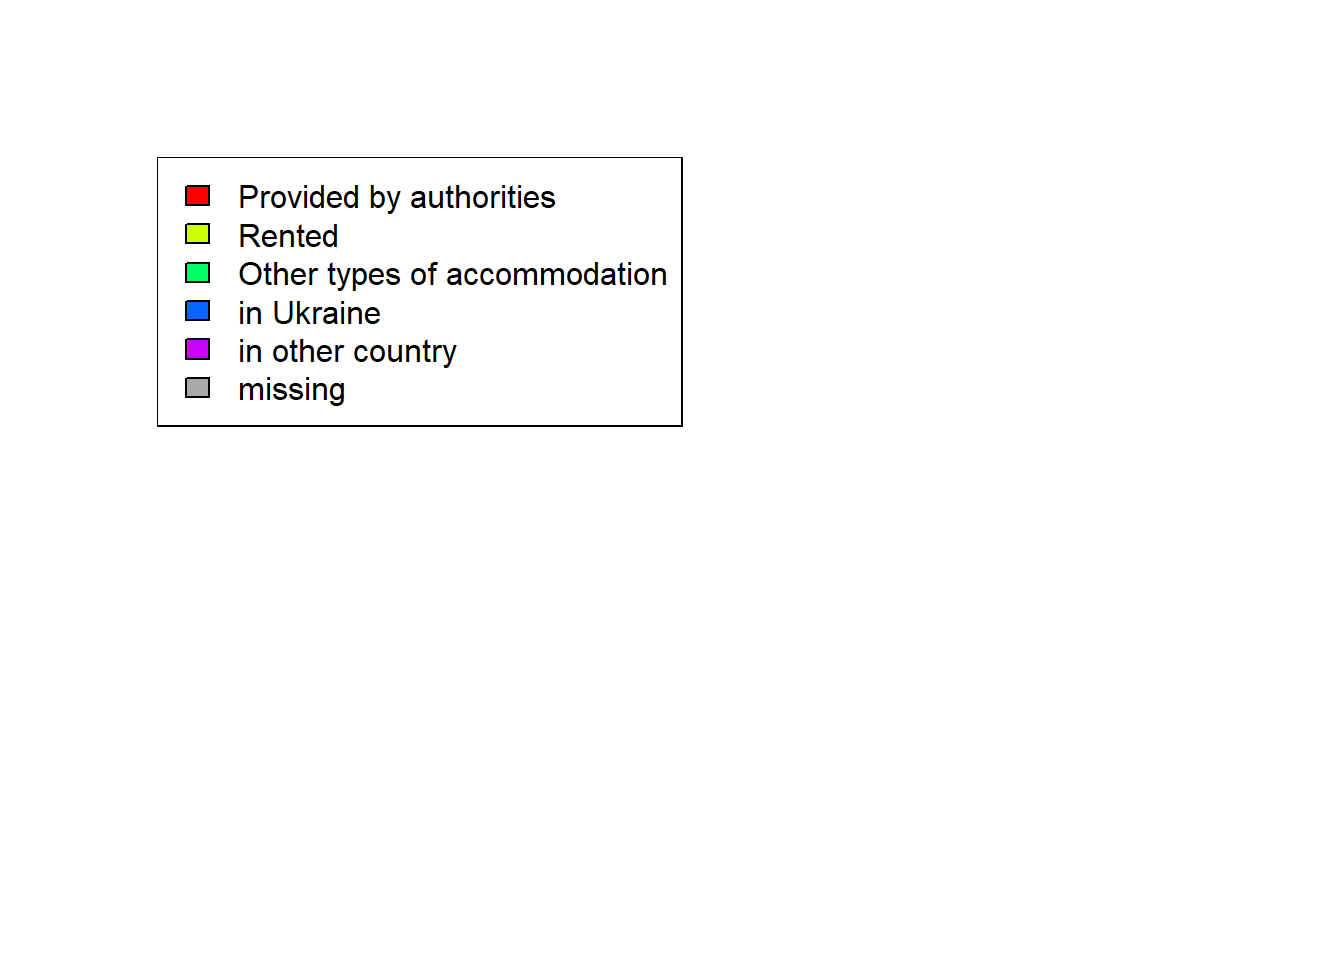
\includegraphics{accommodation_files/figure-pdf/unnamed-chunk-5-1.pdf}

}

\caption{Legend for charts}

\end{figure}%

Frequency tables contain too much information. A graphical
representation allows you to focus on the trajectories that occur most
often. The following graph shows 20 sequences that represent 66.2\% of
all sequences in the data. The frequency of the particular sequence in
the chart corresponds to the height of the row.

\begin{Shaded}
\begin{Highlighting}[]
\FunctionTok{seqfplot}\NormalTok{(}
\NormalTok{  sequence.seq, }\AttributeTok{idxs =} \DecValTok{1}\SpecialCharTok{:}\DecValTok{20}\NormalTok{,}
  \AttributeTok{with.legend =} \ConstantTok{FALSE}\NormalTok{, }\AttributeTok{cex.axis =} \FloatTok{0.65}\NormalTok{,}
  \AttributeTok{border =} \ConstantTok{TRUE}\NormalTok{, }\AttributeTok{pbarw =} \ConstantTok{TRUE}\NormalTok{,}
  \AttributeTok{main =} \StringTok{"Twenty most frequent sequences"}
\NormalTok{)}
\end{Highlighting}
\end{Shaded}

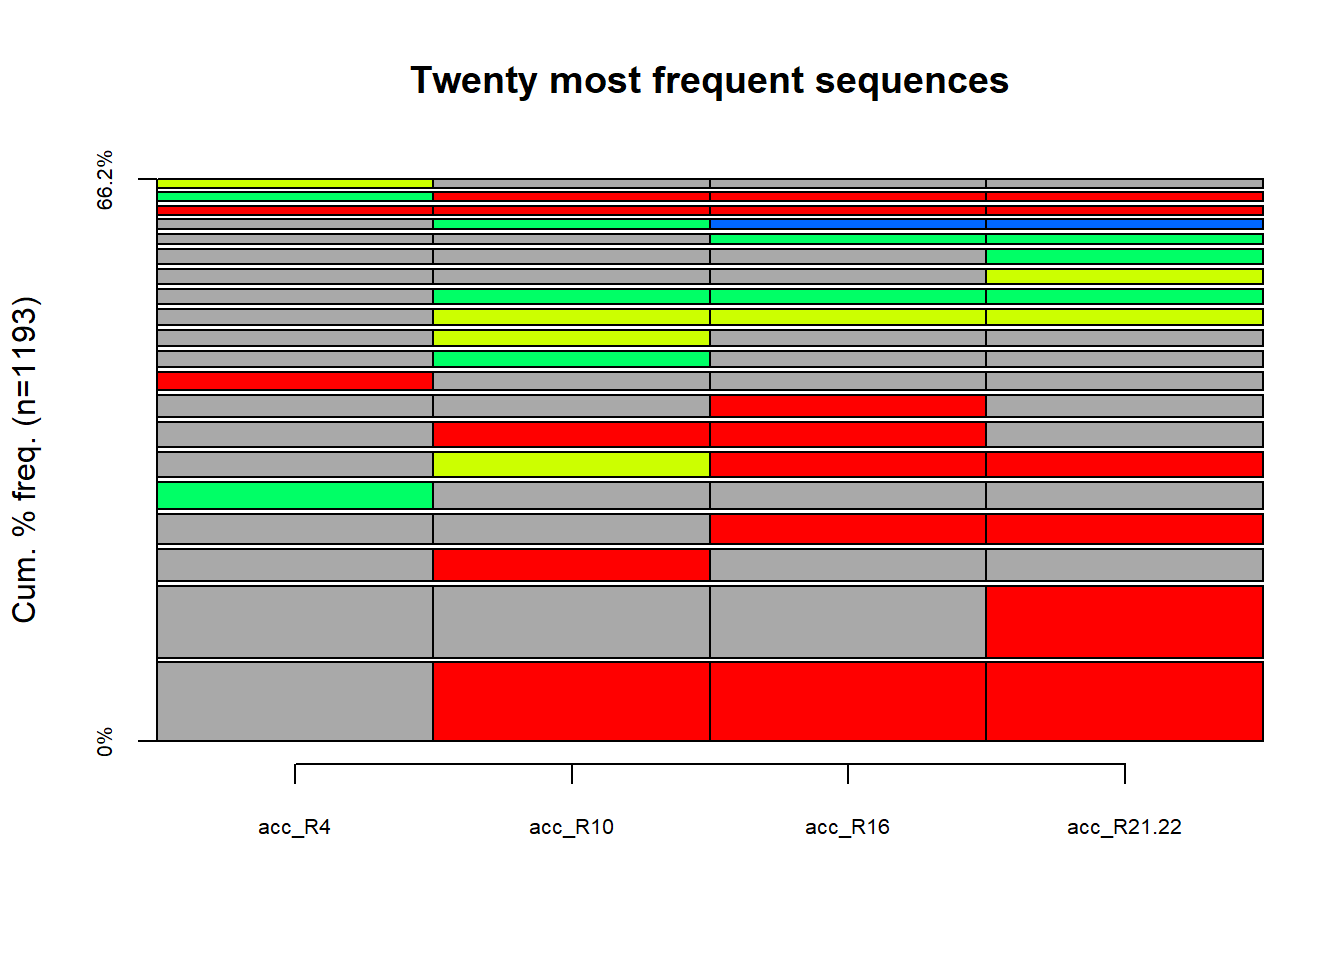
\includegraphics{accommodation_files/figure-pdf/unnamed-chunk-6-1.pdf}

To see all the picture we can plot

\begin{Shaded}
\begin{Highlighting}[]
\FunctionTok{seqplot}\NormalTok{(}
  \AttributeTok{seqdata =}\NormalTok{ sequence.seq, }\AttributeTok{type =} \StringTok{"I"}\NormalTok{, }\CommentTok{\# idxs = 1:100,}
  \AttributeTok{with.legend =} \ConstantTok{FALSE}\NormalTok{, }\AttributeTok{cex.axis =} \FloatTok{0.65}\NormalTok{,}
  \AttributeTok{sortv =} \FunctionTok{sortv}\NormalTok{(sequence.seq, }\AttributeTok{start =} \StringTok{"beg"}\NormalTok{)}
  \CommentTok{\# sortv = tran.seq$acc\_R4}
\NormalTok{)}
\end{Highlighting}
\end{Shaded}

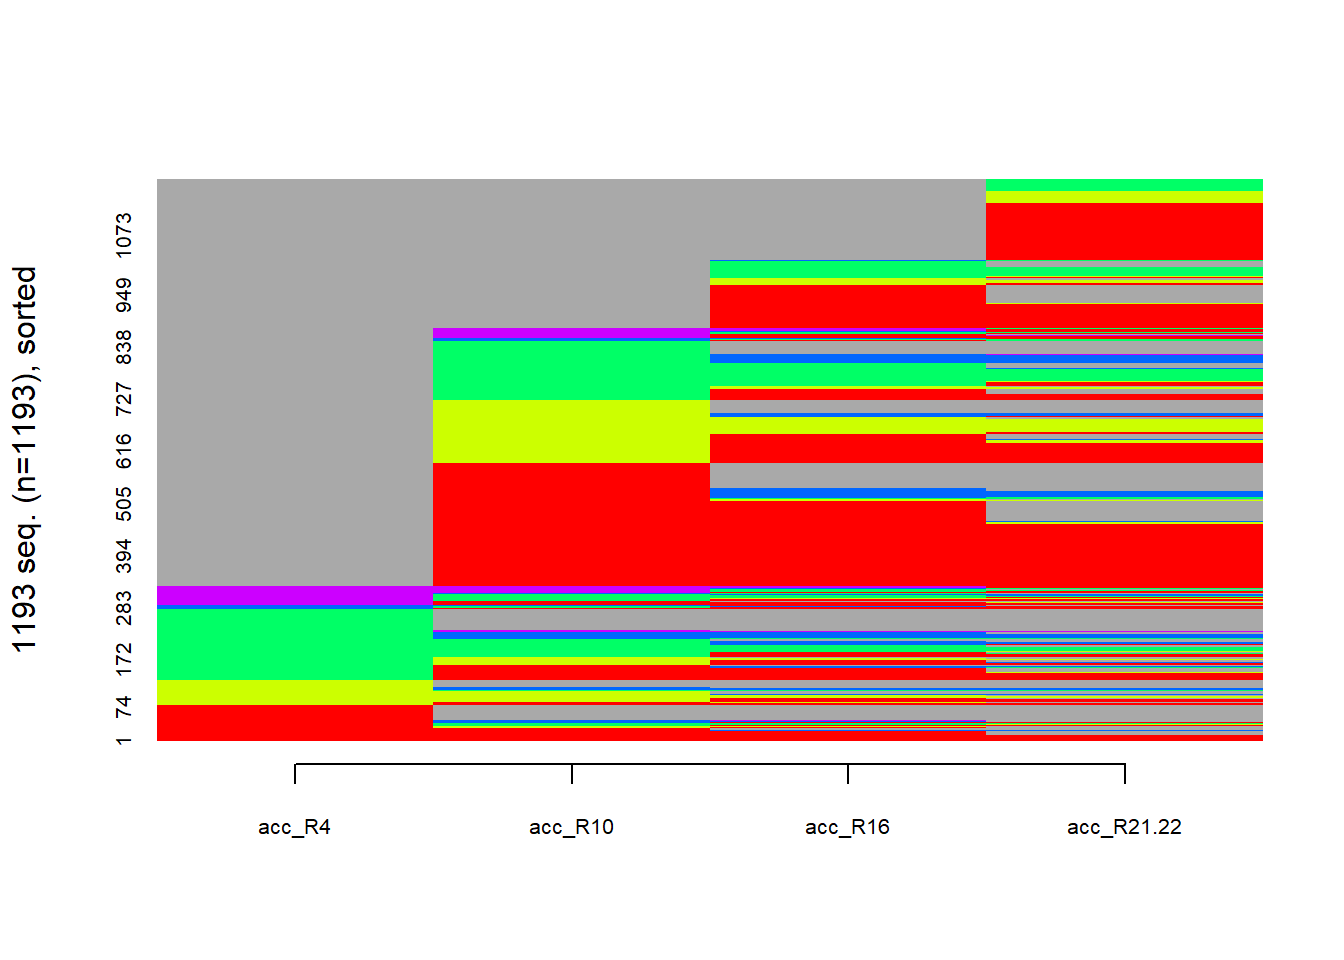
\includegraphics{accommodation_files/figure-pdf/unnamed-chunk-7-1.pdf}

Sorting is possible by final state, which allows you to trace sequences
that end in a specific way. Sorting is also possible by any other
important feature that describes the household.

\begin{Shaded}
\begin{Highlighting}[]
\FunctionTok{seqplot}\NormalTok{(}
  \AttributeTok{seqdata =}\NormalTok{ sequence.seq, }\AttributeTok{type =} \StringTok{"I"}\NormalTok{,}
  \AttributeTok{with.legend =} \ConstantTok{FALSE}\NormalTok{, }\AttributeTok{cex.axis =} \FloatTok{0.65}\NormalTok{,}
  \AttributeTok{sortv =} \FunctionTok{sortv}\NormalTok{(sequence.seq, }\AttributeTok{start =} \StringTok{"end"}\NormalTok{)}
\NormalTok{)}
\end{Highlighting}
\end{Shaded}

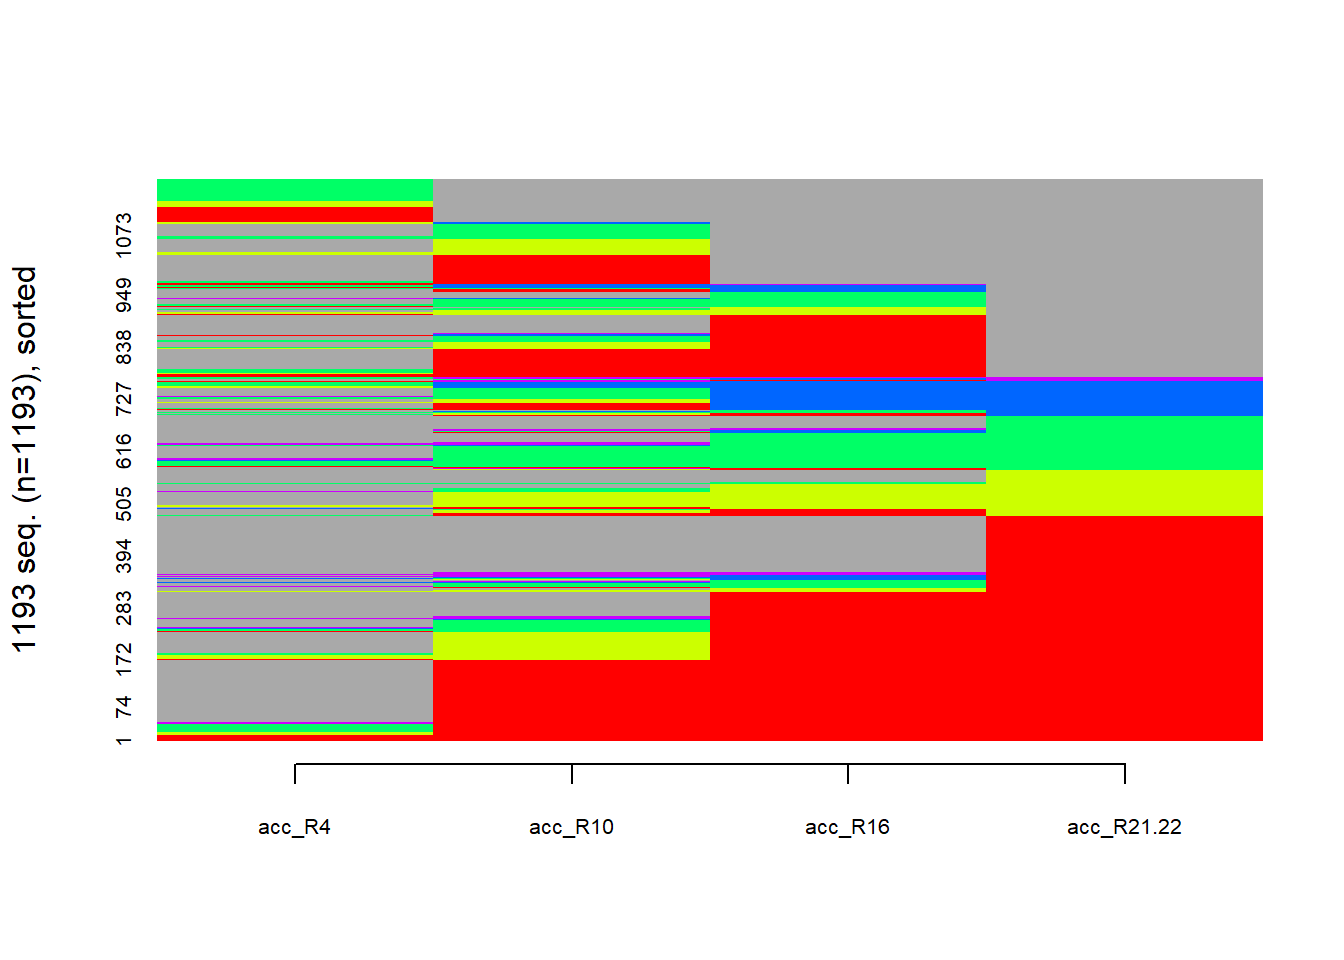
\includegraphics{accommodation_files/figure-pdf/unnamed-chunk-8-1.pdf}

\section{Transition Types}\label{transition-types}

Even after reducing the number of sequence states, there are too many
combinations due to various patterns of missing values to clearly
identify the most important trends. To simplify the analysis, it makes
sense to combine the sequences into groups (types). One approach
proposed in the literature is to use cluster analysis. However, the
hierarchical cluster analysis did not allow me to obtain logical clear
groups, so I decided to go the other way: to classify the sequences
based on the type of transitions from one state to another. To this end,
the number of transitions in our data is first determined:

\begin{Shaded}
\begin{Highlighting}[]
\NormalTok{transitions }\OtherTok{\textless{}{-}} \FunctionTok{as.numeric}\NormalTok{(}\FunctionTok{seqtransn}\NormalTok{(sequence.seq))}

\NormalTok{(tb }\OtherTok{\textless{}{-}} \DecValTok{100} \SpecialCharTok{*} \FunctionTok{prop.table}\NormalTok{(}\FunctionTok{table}\NormalTok{(transitions)))}
\end{Highlighting}
\end{Shaded}

\begin{verbatim}
transitions
        0         1         2         3 
66.890193 25.649623  6.621961  0.838223 
\end{verbatim}

\begin{Shaded}
\begin{Highlighting}[]
\FunctionTok{barplot}\NormalTok{(}
\NormalTok{  tb, }\AttributeTok{col =} \FunctionTok{rainbow}\NormalTok{(}\DecValTok{4}\NormalTok{),}
  \AttributeTok{main =} \StringTok{"Number of transitions"}
\NormalTok{)}
\end{Highlighting}
\end{Shaded}

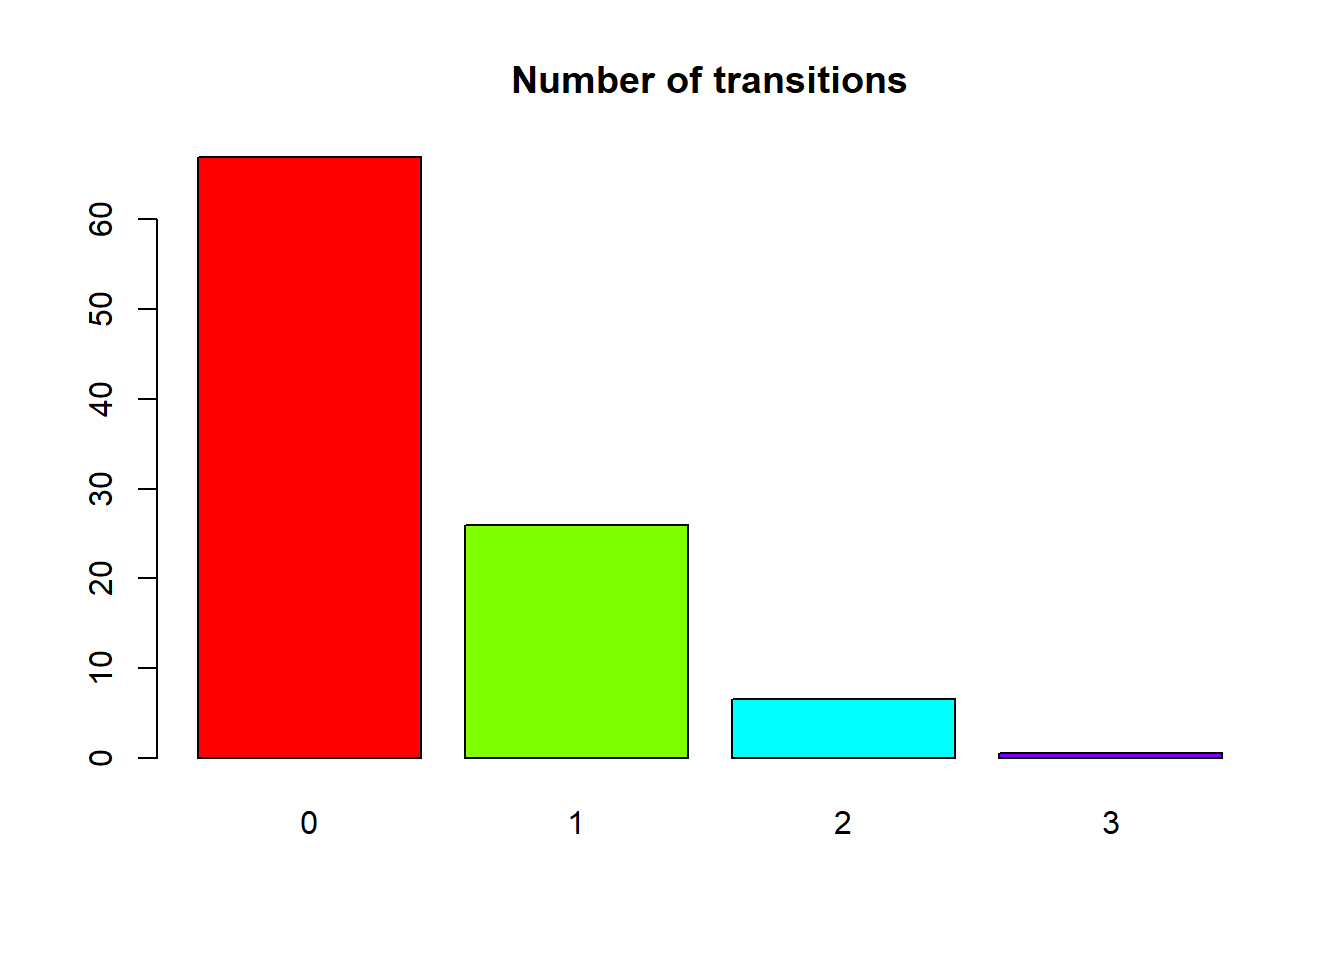
\includegraphics{accommodation_files/figure-pdf/unnamed-chunk-9-1.pdf}

As you can see, the bulk of the sequences are those without transitions,
which can be called stable trajectories.

Now you can distinguish groups of sequences based on the number of
transitions: no transitions, one transition, two transitions, more than
one transition, and so on:

\begin{Shaded}
\begin{Highlighting}[]
\NormalTok{sequence.seq }\SpecialCharTok{\%\textgreater{}\%} 
  \FunctionTok{filter}\NormalTok{(transitions }\SpecialCharTok{==} \DecValTok{0}\NormalTok{) }\OtherTok{{-}\textgreater{}}\NormalTok{ tran0.seq}

\NormalTok{sequence.seq }\SpecialCharTok{\%\textgreater{}\%} 
  \FunctionTok{filter}\NormalTok{(transitions }\SpecialCharTok{==} \DecValTok{1}\NormalTok{) }\OtherTok{{-}\textgreater{}}\NormalTok{ tran1.seq}

\NormalTok{sequence.seq }\SpecialCharTok{\%\textgreater{}\%} 
  \FunctionTok{filter}\NormalTok{(transitions }\SpecialCharTok{==} \DecValTok{2}\NormalTok{) }\OtherTok{{-}\textgreater{}}\NormalTok{ tran2.seq}

\NormalTok{sequence.seq }\SpecialCharTok{\%\textgreater{}\%} 
  \FunctionTok{filter}\NormalTok{(transitions }\SpecialCharTok{\textgreater{}=} \DecValTok{1}\NormalTok{) }\OtherTok{{-}\textgreater{}}\NormalTok{ tran.seq}
\end{Highlighting}
\end{Shaded}

\section{Stable sequences}\label{stable-sequences}

Twenty most frequent sequences cover 93.8\% of time-stable sequences.

\begin{Shaded}
\begin{Highlighting}[]
\NormalTok{tran0.seq }\SpecialCharTok{\%\textgreater{}\%} 
  \FunctionTok{seqfplot}\NormalTok{(}
    \AttributeTok{idxs =} \DecValTok{1}\SpecialCharTok{:}\DecValTok{20}\NormalTok{,}
    \AttributeTok{with.legend =}\NormalTok{ F,}
    \AttributeTok{cex.axis =} \FloatTok{0.65}\NormalTok{,}
    \AttributeTok{pbarw =}\NormalTok{ T,}
    \AttributeTok{main =} \StringTok{"20 stable sequences of accommodation"}
\NormalTok{  )}
\end{Highlighting}
\end{Shaded}

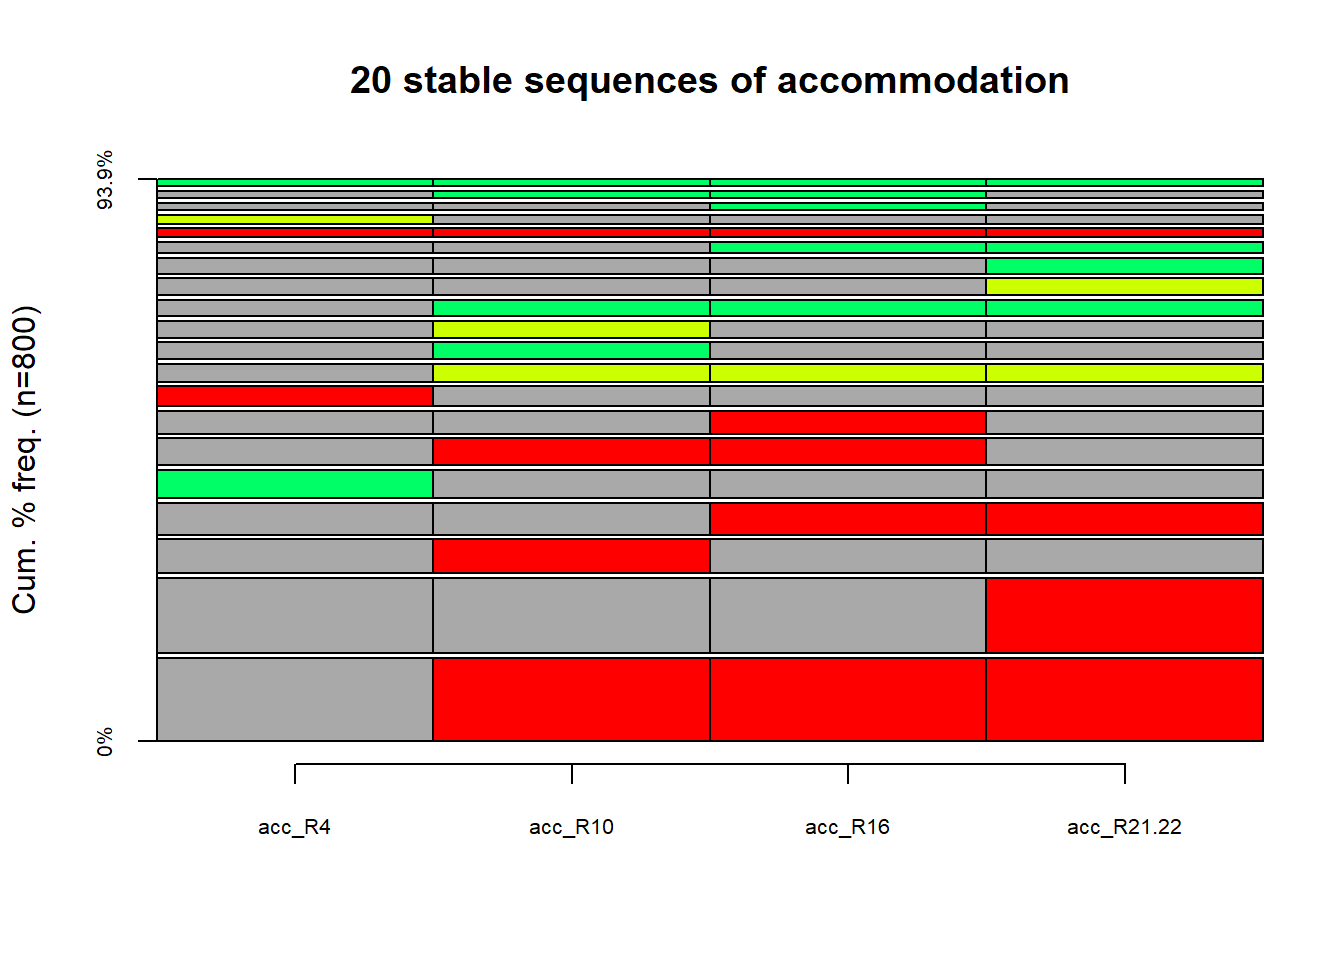
\includegraphics{accommodation_files/figure-pdf/unnamed-chunk-11-1.pdf}

We can simplify the presentation of information about time-stable
sequences by ignoring their differences in the location of missing
values:

\begin{Shaded}
\begin{Highlighting}[]
\DocumentationTok{\#\# Stable frequencies}
\NormalTok{u }\OtherTok{\textless{}{-}}\NormalTok{ tran0.seq}
\NormalTok{u[u }\SpecialCharTok{==} \StringTok{"*"} \SpecialCharTok{|}\NormalTok{ u }\SpecialCharTok{==} \StringTok{"\%"}\NormalTok{] }\OtherTok{\textless{}{-}} \ConstantTok{NA}

\FunctionTok{apply}\NormalTok{(}
  \AttributeTok{X =}\NormalTok{ u, }\AttributeTok{MARGIN =} \DecValTok{1}\NormalTok{, first, }\AttributeTok{na\_rm =} \ConstantTok{TRUE}
\NormalTok{) }\SpecialCharTok{\%\textgreater{}\%}\NormalTok{ sjmisc}\SpecialCharTok{::}\FunctionTok{frq}\NormalTok{()}
\end{Highlighting}
\end{Shaded}

\begin{verbatim}
x <character> 
# total N=798 valid N=798 mean=1.54 sd=0.75

Value  |   N | Raw % | Valid % | Cum. %
---------------------------------------
AUTHOR | 491 | 61.53 |   61.53 |  61.53
OTHACC | 183 | 22.93 |   22.93 |  84.46
RENTED | 124 | 15.54 |   15.54 | 100.00
<NA>   |   0 |  0.00 |    <NA> |   <NA>
\end{verbatim}

Now you can group time-stable sequences by accommodation type in one
chart:

\begin{Shaded}
\begin{Highlighting}[]
\DocumentationTok{\#\# Grouped}
\NormalTok{grp }\OtherTok{\textless{}{-}} \FunctionTok{apply}\NormalTok{(}
  \AttributeTok{X =}\NormalTok{ u, }\AttributeTok{MARGIN =} \DecValTok{1}\NormalTok{, first, }\AttributeTok{na\_rm =} \ConstantTok{TRUE}
\NormalTok{)}

\NormalTok{tran0.seq }\SpecialCharTok{\%\textgreater{}\%} 
  \FunctionTok{seqfplot}\NormalTok{(}
    \AttributeTok{idxs =} \DecValTok{0}\NormalTok{,}
    \AttributeTok{with.legend =} \ConstantTok{TRUE}\NormalTok{, }\AttributeTok{cex.axis =} \FloatTok{0.65}\NormalTok{, }\AttributeTok{pbarw =} \ConstantTok{TRUE}\NormalTok{,}
    \AttributeTok{main =} \StringTok{"Stable accommodation"}\NormalTok{,}
    \AttributeTok{group =}\NormalTok{ grp}
\NormalTok{  )}
\end{Highlighting}
\end{Shaded}

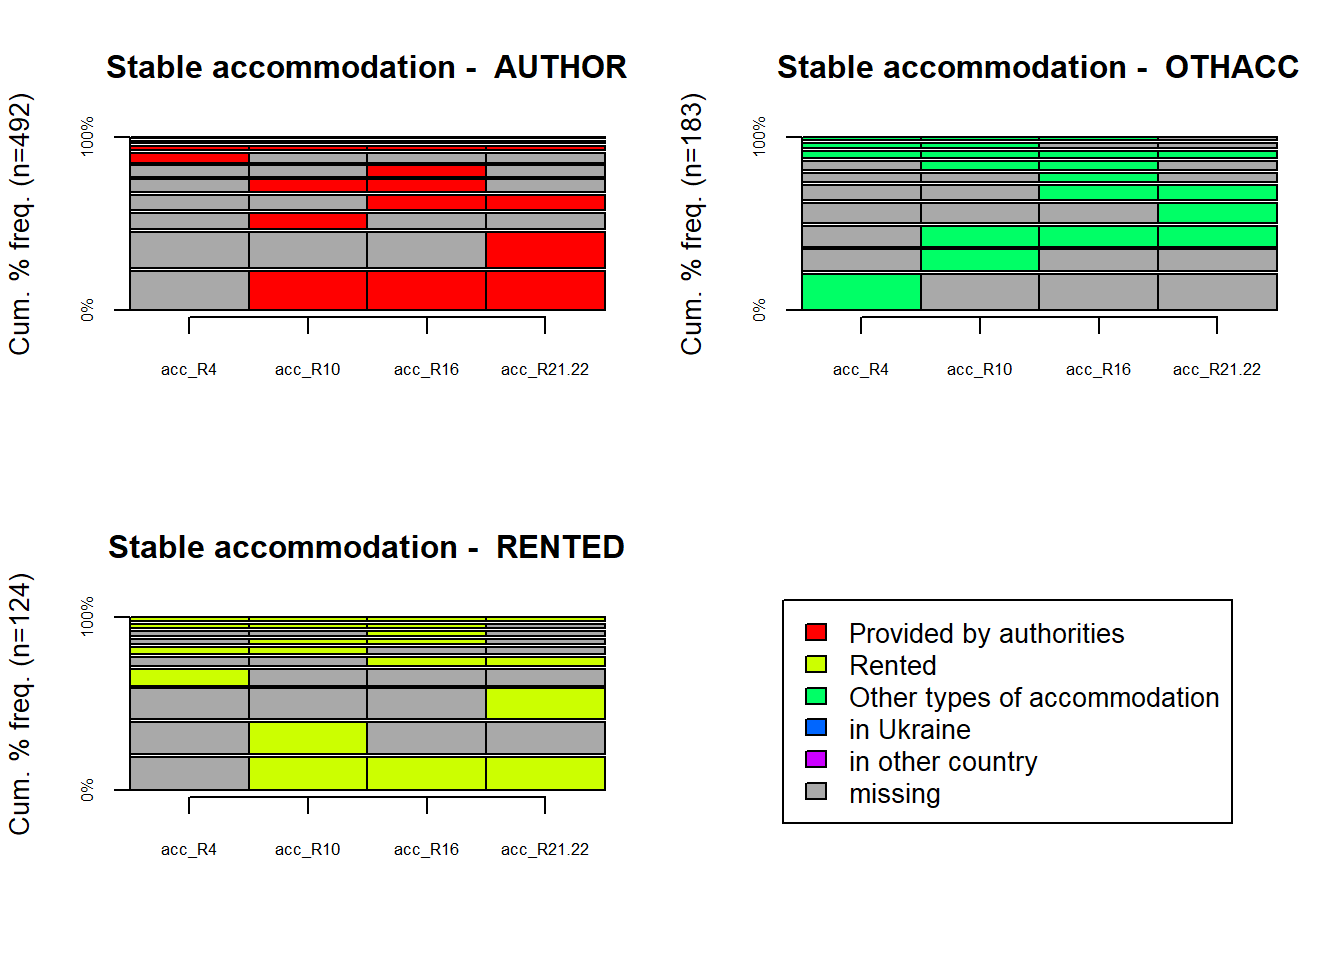
\includegraphics{accommodation_files/figure-pdf/unnamed-chunk-13-1.pdf}

\section{Sequences with transitions}\label{sequences-with-transitions}

Now you can look at sequences with any number of transitions separately.
For example, this table contains sequences with one or more state
transitions:

\begin{Shaded}
\begin{Highlighting}[]
\FunctionTok{seqtab}\NormalTok{(}
\NormalTok{  tran.seq, }\AttributeTok{idxs =} \DecValTok{0}
\NormalTok{)}
\end{Highlighting}
\end{Shaded}

\begin{verbatim}
                                    Freq Percent
*/1-RENTED/1-AUTHOR/2                 44   11.14
*/1-OTHACC/1-IN.UKR/2                 16    4.05
OTHACC/1-AUTHOR/3                     14    3.54
*/1-AUTHOR/1-IN.UKR/2                 13    3.29
*/1-OTHACC/1-AUTHOR/2                 12    3.04
*/1-RENTED/1-AUTHOR/1                 10    2.53
*/1-OTHACC/1-AUTHOR/1                  9    2.28
*/1-OTHACC/2-AUTHOR/1                  9    2.28
OTHACC/1-AUTHOR/2                      9    2.28
OTHACC/1-IN.UKR/3                      8    2.03
OTHACC/2-AUTHOR/2                      8    2.03
*/1-OTHACC/1-RENTED/2                  7    1.77
RENTED/2-AUTHOR/2                      7    1.77
*/1-AUTHOR/1-IN.UKR/1                  6    1.52
*/1-RENTED/1-IN.UKR/2                  6    1.52
*/1-IN.OTH/2-AUTHOR/1                  5    1.27
*/1-RENTED/1-AUTHOR/1-RENTED/1         5    1.27
IN.OTH/2-OTHACC/2                      5    1.27
OTHACC/1-IN.UKR/2                      5    1.27
OTHACC/1-RENTED/1-AUTHOR/2             5    1.27
RENTED/1-AUTHOR/3                      5    1.27
*/2-RENTED/1-AUTHOR/1                  4    1.01
IN.OTH/1-AUTHOR/3                      4    1.01
IN.OTH/1-OTHACC/1-AUTHOR/2             4    1.01
IN.OTH/3-AUTHOR/1                      4    1.01
OTHACC/1-RENTED/1-AUTHOR/1             4    1.01
OTHACC/2-AUTHOR/1                      4    1.01
OTHACC/2-IN.UKR/2                      4    1.01
RENTED/1-IN.UKR/3                      4    1.01
*/1-AUTHOR/1-RENTED/2                  3    0.76
*/1-AUTHOR/2-RENTED/1                  3    0.76
*/1-IN.OTH/1-OTHACC/2                  3    0.76
*/1-IN.OTH/2-OTHACC/1                  3    0.76
*/1-RENTED/2-AUTHOR/1                  3    0.76
AUTHOR/2-IN.UKR/2                      3    0.76
OTHACC/1-AUTHOR/1                      3    0.76
RENTED/1-IN.UKR/1                      3    0.76
*/1-AUTHOR/1-OTHACC/2                  2    0.51
*/1-AUTHOR/2-IN.UKR/1                  2    0.51
*/1-IN.OTH/1-AUTHOR/1                  2    0.51
*/1-IN.OTH/1-AUTHOR/2                  2    0.51
*/1-IN.OTH/1-OTHACC/1-AUTHOR/1         2    0.51
*/1-OTHACC/1-IN.UKR/1-IN.OTH/1         2    0.51
*/1-OTHACC/1-RENTED/1                  2    0.51
*/1-RENTED/1-AUTHOR/1-IN.UKR/1         2    0.51
*/2-OTHACC/1-AUTHOR/1                  2    0.51
*/2-OTHACC/1-IN.UKR/1                  2    0.51
*/2-OTHACC/1-RENTED/1                  2    0.51
AUTHOR/1-IN.UKR/2                      2    0.51
AUTHOR/1-RENTED/1-AUTHOR/1             2    0.51
AUTHOR/1-RENTED/1-AUTHOR/2             2    0.51
IN.OTH/1-OTHACC/1-RENTED/2             2    0.51
IN.OTH/1-OTHACC/3                      2    0.51
IN.UKR/1-OTHACC/3                      2    0.51
OTHACC/1-IN.OTH/3                      2    0.51
*/1-AUTHOR/1-IN.UKR/1-OTHACC/1         1    0.25
*/1-AUTHOR/1-OTHACC/1-AUTHOR/1         1    0.25
*/1-AUTHOR/1-RENTED/1                  1    0.25
*/1-AUTHOR/1-RENTED/1-AUTHOR/1         1    0.25
*/1-AUTHOR/2-IN.OTH/1                  1    0.25
*/1-IN.OTH/1-AUTHOR/1-IN.OTH/1         1    0.25
*/1-IN.OTH/1-AUTHOR/1-OTHACC/1         1    0.25
*/1-IN.OTH/1-IN.UKR/1-AUTHOR/1         1    0.25
*/1-IN.OTH/1-IN.UKR/1-OTHACC/1         1    0.25
*/1-IN.OTH/1-OTHACC/1-IN.OTH/1         1    0.25
*/1-IN.UKR/1-AUTHOR/1                  1    0.25
*/1-IN.UKR/1-AUTHOR/1-OTHACC/1         1    0.25
*/1-IN.UKR/1-AUTHOR/2                  1    0.25
*/1-IN.UKR/1-OTHACC/1-AUTHOR/1         1    0.25
*/1-IN.UKR/1-OTHACC/1-IN.UKR/1         1    0.25
*/1-IN.UKR/1-OTHACC/2                  1    0.25
*/1-IN.UKR/2-AUTHOR/1                  1    0.25
*/1-OTHACC/1-AUTHOR/1-RENTED/1         1    0.25
*/1-OTHACC/1-IN.UKR/1-OTHACC/1         1    0.25
*/1-OTHACC/1-RENTED/1-IN.UKR/1         1    0.25
*/1-OTHACC/2-IN.UKR/1                  1    0.25
*/1-RENTED/1-AUTHOR/1-OTHACC/1         1    0.25
*/1-RENTED/1-IN.UKR/1                  1    0.25
*/1-RENTED/1-IN.UKR/1-AUTHOR/1         1    0.25
*/1-RENTED/2-IN.UKR/1                  1    0.25
*/2-AUTHOR/1-IN.OTH/1                  1    0.25
*/2-AUTHOR/1-RENTED/1                  1    0.25
*/2-IN.OTH/1-OTHACC/1                  1    0.25
*/2-IN.UKR/1-OTHACC/1                  1    0.25
AUTHOR/1-IN.OTH/1-IN.UKR/2             1    0.25
AUTHOR/1-IN.UKR/1-AUTHOR/2             1    0.25
AUTHOR/1-IN.UKR/1-IN.OTH/1             1    0.25
AUTHOR/1-IN.UKR/3                      1    0.25
AUTHOR/1-OTHACC/1-AUTHOR/2             1    0.25
AUTHOR/1-OTHACC/1-IN.OTH/1-AUTHOR/1    1    0.25
AUTHOR/1-OTHACC/1-IN.UKR/1-OTHACC/1    1    0.25
AUTHOR/1-OTHACC/2                      1    0.25
AUTHOR/1-OTHACC/2-RENTED/1             1    0.25
AUTHOR/1-OTHACC/3                      1    0.25
AUTHOR/1-RENTED/2                      1    0.25
AUTHOR/1-RENTED/3                      1    0.25
IN.OTH/1-AUTHOR/1                      1    0.25
IN.OTH/1-AUTHOR/1-IN.UKR/1             1    0.25
IN.OTH/1-AUTHOR/2-RENTED/1             1    0.25
IN.OTH/1-IN.UKR/1-IN.OTH/1-AUTHOR/1    1    0.25
IN.OTH/1-IN.UKR/1-OTHACC/1             1    0.25
IN.OTH/1-IN.UKR/2-AUTHOR/1             1    0.25
IN.OTH/1-OTHACC/1-IN.OTH/2             1    0.25
IN.OTH/1-OTHACC/1-IN.UKR/1-AUTHOR/1    1    0.25
IN.OTH/1-OTHACC/1-IN.UKR/2             1    0.25
IN.OTH/1-OTHACC/2-AUTHOR/1             1    0.25
IN.OTH/1-OTHACC/2-IN.UKR/1             1    0.25
IN.OTH/1-RENTED/2-AUTHOR/1             1    0.25
IN.OTH/2-AUTHOR/1                      1    0.25
IN.OTH/2-AUTHOR/2                      1    0.25
IN.OTH/2-IN.UKR/1-AUTHOR/1             1    0.25
IN.OTH/2-IN.UKR/1-OTHACC/1             1    0.25
IN.OTH/2-OTHACC/1                      1    0.25
IN.OTH/2-OTHACC/1-AUTHOR/1             1    0.25
IN.UKR/1-AUTHOR/1-RENTED/2             1    0.25
IN.UKR/1-AUTHOR/3                      1    0.25
IN.UKR/1-OTHACC/1-AUTHOR/2             1    0.25
IN.UKR/1-OTHACC/1-IN.UKR/1-AUTHOR/1    1    0.25
IN.UKR/1-OTHACC/1-IN.UKR/1-OTHACC/1    1    0.25
IN.UKR/2-AUTHOR/1                      1    0.25
IN.UKR/2-OTHACC/1-AUTHOR/1             1    0.25
OTHACC/1-AUTHOR/1-IN.UKR/1-OTHACC/1    1    0.25
OTHACC/1-AUTHOR/1-IN.UKR/2             1    0.25
OTHACC/1-AUTHOR/1-RENTED/1             1    0.25
OTHACC/1-AUTHOR/2-IN.UKR/1             1    0.25
OTHACC/1-AUTHOR/2-RENTED/1             1    0.25
OTHACC/1-IN.OTH/1                      1    0.25
OTHACC/1-IN.OTH/1-OTHACC/1             1    0.25
OTHACC/1-IN.OTH/1-OTHACC/1-IN.OTH/1    1    0.25
OTHACC/1-IN.UKR/1-IN.OTH/1-OTHACC/1    1    0.25
OTHACC/1-IN.UKR/1-OTHACC/2             1    0.25
OTHACC/1-IN.UKR/2-AUTHOR/1             1    0.25
OTHACC/1-RENTED/1                      1    0.25
OTHACC/1-RENTED/1-AUTHOR/1-IN.UKR/1    1    0.25
OTHACC/1-RENTED/1-IN.UKR/2             1    0.25
OTHACC/1-RENTED/3                      1    0.25
OTHACC/2-AUTHOR/1-OTHACC/1             1    0.25
OTHACC/2-AUTHOR/1-RENTED/1             1    0.25
OTHACC/2-IN.UKR/1                      1    0.25
OTHACC/2-IN.UKR/1-AUTHOR/1             1    0.25
OTHACC/2-RENTED/1                      1    0.25
OTHACC/3-IN.UKR/1                      1    0.25
OTHACC/3-RENTED/1                      1    0.25
RENTED/1-AUTHOR/1-RENTED/1             1    0.25
RENTED/1-AUTHOR/2                      1    0.25
RENTED/1-IN.UKR/1-AUTHOR/2             1    0.25
RENTED/1-OTHACC/3                      1    0.25
RENTED/2-AUTHOR/1                      1    0.25
RENTED/2-IN.UKR/2                      1    0.25
RENTED/3-AUTHOR/1                      1    0.25
\end{verbatim}

The most informative way to represent such sequences is in the form of a
table of transitions between individual states. Such tables can also be
built for transitions between individual rounds:

\begin{Shaded}
\begin{Highlighting}[]
\DocumentationTok{\#\# Table of transitions}
\FunctionTok{seqtrate}\NormalTok{(tran1.seq, }\AttributeTok{with.missing =} \ConstantTok{TRUE}\NormalTok{) }\SpecialCharTok{\%\textgreater{}\%}  \CommentTok{\# , time.varying = TRUE}
  \FunctionTok{round}\NormalTok{(}\AttributeTok{digits =} \DecValTok{2}\NormalTok{)}
\end{Highlighting}
\end{Shaded}

\begin{verbatim}
 [>] computing transition probabilities for states AUTHOR/RENTED/OTHACC/IN.UKR/IN.OTH/* ...
\end{verbatim}

\begin{verbatim}
            [-> AUTHOR] [-> RENTED] [-> OTHACC] [-> IN.UKR] [-> IN.OTH] [-> *]
[AUTHOR ->]        0.62        0.04        0.02        0.12        0.01   0.19
[RENTED ->]        0.59        0.23        0.01        0.12        0.00   0.05
[OTHACC ->]        0.38        0.08        0.30        0.21        0.02   0.01
[IN.UKR ->]        0.05        0.00        0.04        0.74        0.00   0.17
[IN.OTH ->]        0.31        0.00        0.23        0.00        0.44   0.02
[* ->]             0.16        0.33        0.30        0.02        0.08   0.11
\end{verbatim}

You can visualize transition tables using heatmaps:

\begin{Shaded}
\begin{Highlighting}[]
\FunctionTok{seqtrate}\NormalTok{(tran.seq, }\AttributeTok{with.missing =} \ConstantTok{TRUE}\NormalTok{) }\SpecialCharTok{\%\textgreater{}\%} 
  \FunctionTok{round}\NormalTok{(}\AttributeTok{digits =} \DecValTok{2}\NormalTok{) }\SpecialCharTok{\%\textgreater{}\%} 
\NormalTok{  corrplot}\SpecialCharTok{::}\FunctionTok{corrplot}\NormalTok{(}
    \AttributeTok{method =} \StringTok{"square"}\NormalTok{, }\AttributeTok{is.corr =} \ConstantTok{FALSE}\NormalTok{, }\AttributeTok{addCoef.col =} \StringTok{"blue"}
\NormalTok{  )}
\end{Highlighting}
\end{Shaded}

\begin{verbatim}
 [>] computing transition probabilities for states AUTHOR/RENTED/OTHACC/IN.UKR/IN.OTH/* ...
\end{verbatim}

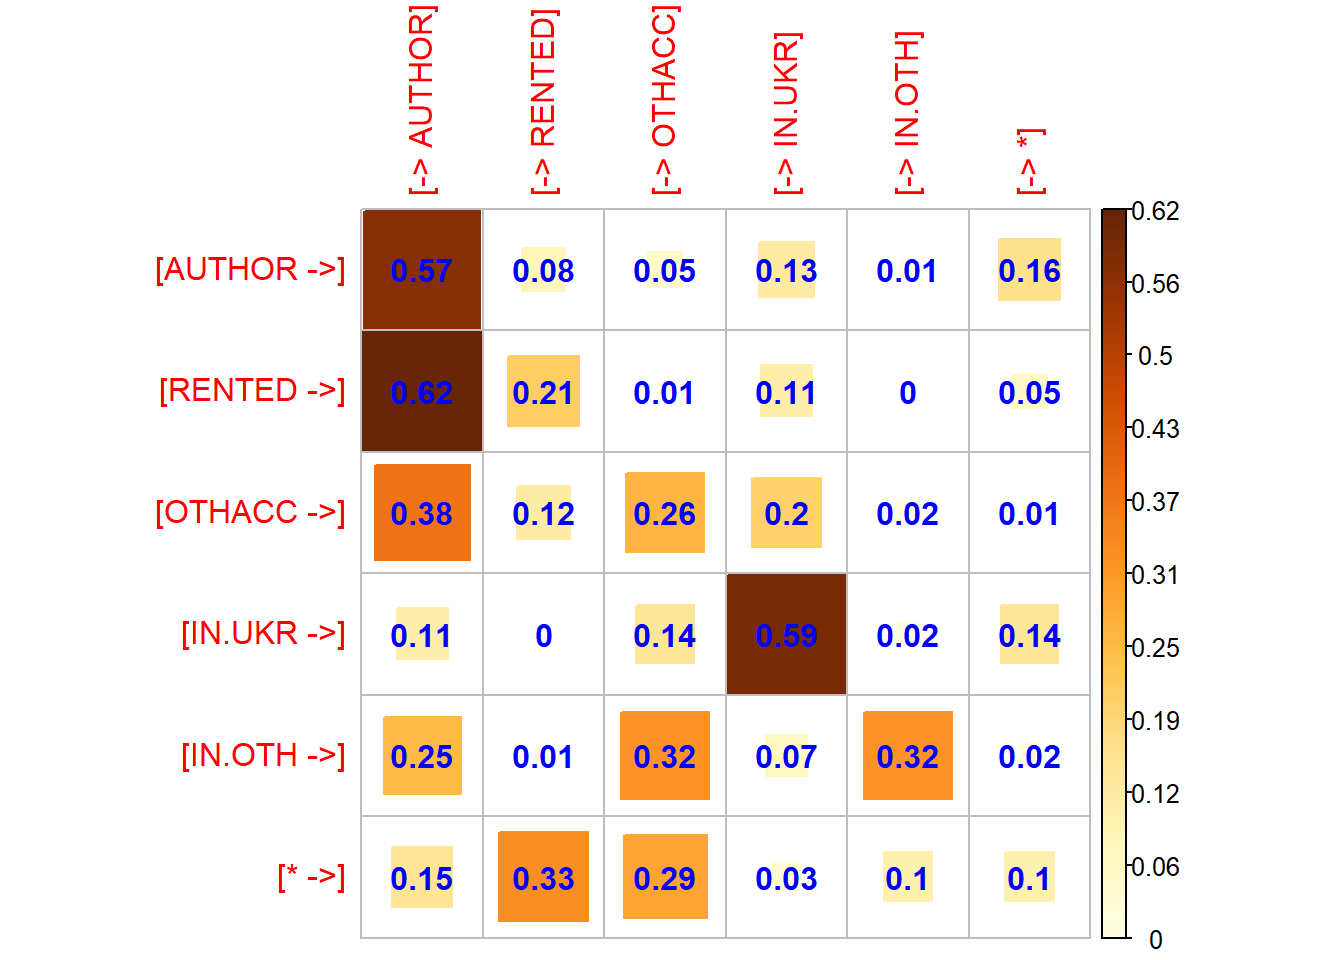
\includegraphics{accommodation_files/figure-pdf/unnamed-chunk-16-1.pdf}

A chronograph chart shows the dynamics of state distributions between
rounds for sequences with transitions:

\begin{Shaded}
\begin{Highlighting}[]
\FunctionTok{seqdplot}\NormalTok{(}
\NormalTok{  tran.seq, }\AttributeTok{main =} \StringTok{"State distribution plot (transitions)"}\NormalTok{,}
  \AttributeTok{with.legend =}\NormalTok{ F, }\AttributeTok{cex.axis =} \FloatTok{0.65}
\NormalTok{)}
\end{Highlighting}
\end{Shaded}

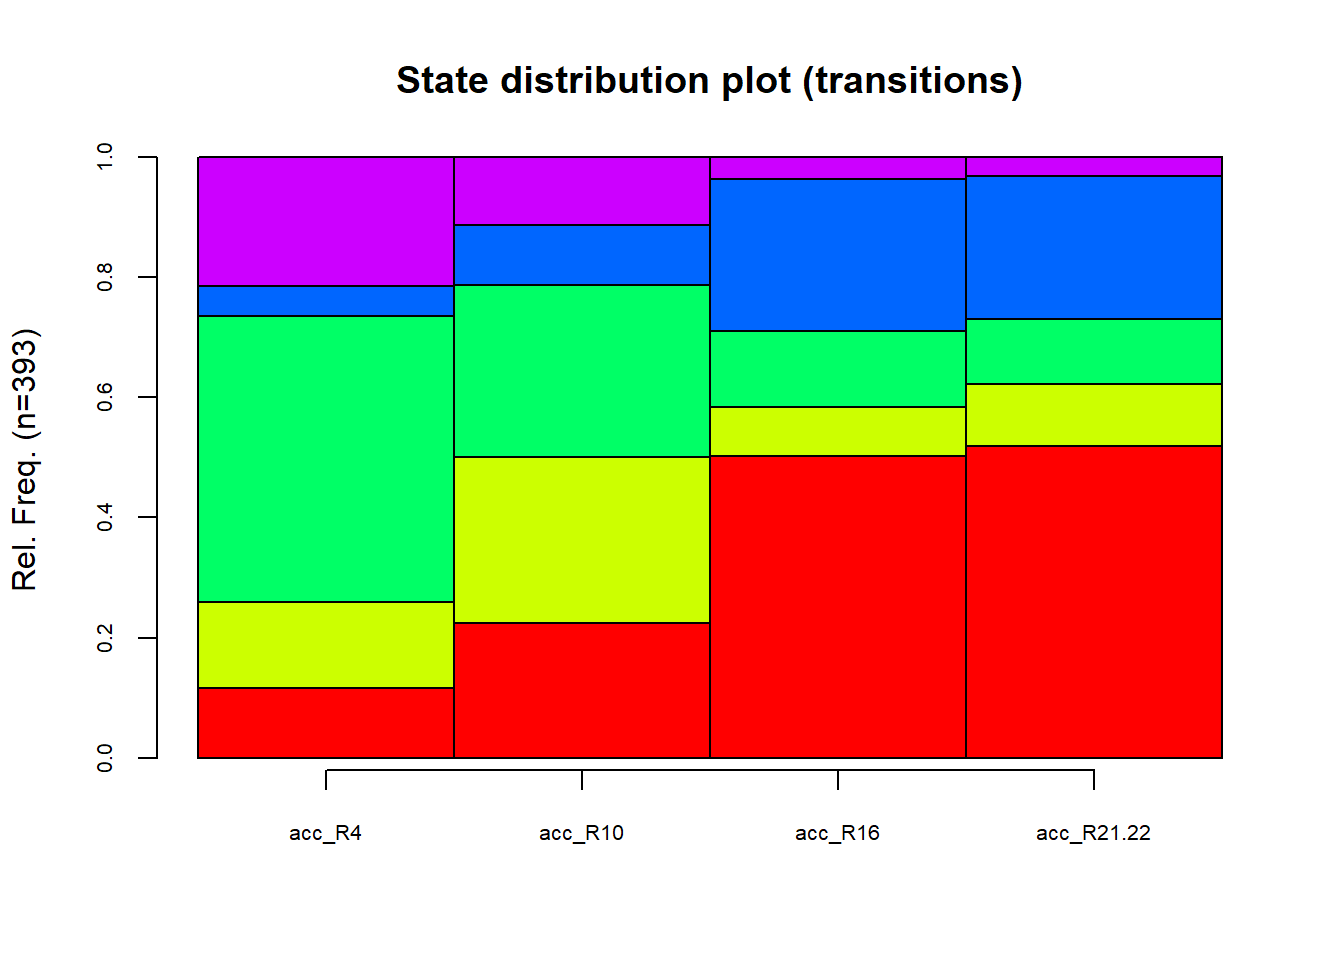
\includegraphics{accommodation_files/figure-pdf/unnamed-chunk-17-1.pdf}

\bookmarksetup{startatroot}

\chapter{Summary}\label{summary}

In summary, this book has no content whatsoever.

\begin{Shaded}
\begin{Highlighting}[]
\DecValTok{1} \SpecialCharTok{+} \DecValTok{1}
\end{Highlighting}
\end{Shaded}

\begin{verbatim}
[1] 2
\end{verbatim}

\bookmarksetup{startatroot}

\chapter*{References}\label{references}
\addcontentsline{toc}{chapter}{References}

\markboth{References}{References}

\phantomsection\label{refs}
\begin{CSLReferences}{0}{1}
\end{CSLReferences}



\end{document}
